\documentclass[letterpaper,12pt]{article} % Documento en dos columnas, tamaño carta
\usepackage[spanish]{babel}       % Traduce capítulos, fechas, etc. al español
\usepackage[utf8]{inputenc}       % Permite usar acentos directamente
\usepackage[T1]{fontenc}          % Codificación para que se vean bien los caracteres en PDF
\usepackage{lmodern}              % Usa fuentes escalables compatibles con microtype
\usepackage{geometry}             % Control de márgenes y tamaño de página
\usepackage{fancyhdr}            % Encabezados y pies de página personalizados


%Notación 

\usepackage{amsmath}  % Ecuaciones, símbolos y fuentes matemáticas
\usepackage{amssymb}
\usepackage{amsfonts}
\usepackage{siunitx}                     % Escritura coherente de unidades del SI y números

%gráficos 

\usepackage{graphicx}           % Insertar y escalar imágenes
\usepackage{subcaption}         % Subfiguras dentro de una figura
\usepackage{booktabs}           % Tablas más profesionales
\usepackage{longtable}          % Tablas que ocupan varias páginas
\usepackage{tabularx}           % Tablas con ancho ajustable automáticamente
\usepackage{array}              % Mejoras en tablas y alineación de columnas


% --- COLORES Y LISTAS PERSONALIZADAS ---
\usepackage{xcolor}             % Uso de colores en texto y figuras
\usepackage{enumitem}           % Listas personalizadas (espaciado, numeración)

% --- HIPERVÍNCULOS Y NAVEGACIÓN ---
\usepackage[hidelinks]{hyperref}           % Enlaces ciclables en PDF (índice, URLs, referencias)

% --- DIAGRAMAS TÉCNICOS ---
\usepackage{tikz}                         % Gráficos vectoriales (bloques, flujos, redes)
\usepackage{forest}                      % Árboles, jerarquías (estructuras)

% --- ALGORITMOS Y CÓDIGO FUENTE ---
\usepackage{algorithm2e}    % Pseudocódigo paso a paso (algoritmos)
\usepackage{listings}       % Mostrar código fuente con formato

\geometry{letterpaper, margin=1in} % Márgenes de 1 pul
\title{Ayahuik 1: Guía de Misión}
\author{CUAUHTÉMOC IPN}


\pagestyle{fancy} 
\setlength{\headheight}{14.5pt}
\fancyhf{}
\fancyhead[C]{Cuauhtemoc IPN}
\fancyhead[R]{AYAHUIK 1}
\fancyhead[L]{Guia de Misión}
\fancyfoot[R]{\thepage}

\graphicspath{{Imagenes/}}

\begin{document}

\tableofcontents

\section{Antecedentes}

    \subsection{Antecedentes Históricos}

    \subsection{Antecedentes IPN}

    \subsection{Antecedentes Cuauhtémoc IPN}

\section{Descripción general de la misión}

    \subsection{Participantes de la misión}

    \subsection{CONOPS}

    \subsection{Descripción de la carga util}

    \subsection{Descripción del proceso de diseño y construcción}

    \subsection{Descripción del lanzamiento y recuperación}

\section{Objetivos y criterios de éxito}

    \subsection{Objetivos generales}
    La misión Ayahuik 1 tiene como objetivo principal el desarrollo de una carga util capaz de ser lanzada a la estratósfera
    y recuperar parametros atmosféricos y de condiciones del aire a diferentes alturas,
    así como la obtención de material fotográfico y de video del lanzamiento y vuelo de la misma.


    Esto con el fin de la obtencion de datos cientificos como de divulgacion.

    \subsection{Objetivos específicos}
    \begin{itemize}
        \item El desarollo de una carga util de un globo sonda la cual demuesre las capacidadesde desarollo tecnologico de los miembros del equipo Cuauhtémoc IPN.
        \item Fotografia y video de las zonas aledañas al volcan Popocatepetl.
        \item Sondeo de gases en diferentes altitudes en las zonas aledañas al volcan Popocatepetl.
        \item Recolección de datos atmosféricos y de condiciones del aire a diferentes alturas
        \item Capacitacion de las nuevas generaciones del equipo tanto en ambitos tecnologicos como de documentación y divulgacion.
        \item Incentivacion del desarollo de nuevas tecnologias y retos para los miembros del equipo.
        \item Divulgacion cientifica con los datos y videos obtenidos al vuelo.
        
    \end{itemize}    

    \newpage
    
    \subsection{Criterios de éxito}

    Los criterios de exito de la mision se basaran en una ponderacion al 100\% de los hitos obtenidos durante el desarollo de la mision en su etapa de vuelo dependiendo de su importancia y complejidad los cuales son desarollados a continuacion:

    \begin{longtable}{|m{4.3cm}|c|c|c|}
    \hline
    \textbf{Criterio de Extito} & \textbf{Puntos maximos} & \textbf{Puntos Obtenidos} & \textbf{Observaciones} \\
    \hline
    \endfirsthead
    \hline
    \textbf{Criterio de Extito} & \textbf{Puntos maximos} & \textbf{Puntos Obtenidos} & \textbf{Observaciones} \\
    \hline
    \endhead
    Vuelo a grandes altitudes & 10 &  & \\
    \midrule
    Medicion de temperatura en vuelo & 10 &  & \\
    \midrule
    Medicion de la presion en vuelo & 10 &  & \\
    \midrule
    Meidicion de oxigeno en vuelo & 10 &  & \\
    \midrule
    Medicion de vapor de agua en vuelo & 10 &  & \\
    \midrule
    Medicion de $CO_{2}$ en vuelo & 10 &  & \\
    \midrule
    Medicion de $SO_{2}$ en vuelo & 10 &  & \\
    \midrule
    Medicion de $H_{2}$ en vuelo   \phantom{text} & 10 &  & \\
    \midrule
    Toma de fotografia del Popocatepetl & 10 &  & \\
    \midrule
    Toma de video del Popocatepetl & 10 &  & \\
    \midrule
    Toma de fotografia del horizonte & 10 &  & \\
    \midrule
    Toma de video del horizonte & 10 &  & \\
    \midrule
    Recepcion de telemetria por RF & 10 &  & \\
    \midrule
    Recepcion de telemetria por SMS & 10 &  & \\
    \midrule
    Recepcion de telemetria por MSM & 10 &  & \\
    \midrule
    Descenso con control autonomo & 10 &  & \\
    \midrule
    Funcionamiento de la Estacion Terrena & 10 &  & \\
    \midrule
    Funcionamiento de la computadora de vuelo & 10 &  & \\
    \midrule
    Funcionamiento de la electronica & 10 &  & \\
    \midrule
    Señal GPS constante de vuelo & 10 &  & \\
    \midrule
    Recuperacion de la carga util & 10 &  & \\
    \midrule
    Estado de la carga util al recuperar & 10 &  & \\
    \midrule
    \textbf{TOTAL} & 220 &  & -\\
    \hline
    \end{longtable}

    Por lo tanto el porcentaje de exito de la mision es de: $\%$

    \newpage

\section{Resultados esperados}

    La misión contara con diferentes resultados esperados, los cuales se dividen en resultados técnicos, de la carga util y de la misión en general, 
    los cuales validaran el correcto desarrollo y éxito total o parcial de la misión.

    \subsection{Resultados técnicos}

    documentación técnica de la carga util y sistemas asi como del desarrollo de los mismos
    (PDR, CDR y PFR).
    Asimismo un documento con los resultados de las pruebas ambientales realizadas (vació, térmica, vibraciones y drop test)
    detallando el desempeño de la carga util y validando a la misma para su lanzamiento. 

    \subsection{Resultados de la carga útil}

    Carga util reutilizable que cumpla con todos los requisitos establecidos para la misión, la cual
    demuestre tener capacidades de recolección de datos y transmisión de los mismos tanto por radio
    frecuencia como por SMS y MSM a una estación terrena.
    
    Esta deberá contar con manual de operaciones 
    para la correcta operación y recuperación de la carga util.
    
    La misma deberá ser capaz de resistir las condiciones de lanzamiento y vuelo con condiciones extremas de presión y temperatura,
    asi como de ser capaz de soportar el retorno a tierra y ser recuperada en condiciones de operatividad.


    \subsection{Resultados de la misión}

    Obtención de datos atmosféricos y de condiciones del aire a diferentes alturas de gran utilidad
    científica y de investigación, asi como material fotográfico y de video del lanzamiento y vuelo desde la carga util.
    
    Aprendizaje y capacitación practica para la nueva generación del equipo Cuauhtémoc IPN 2025-2026 a lo largo de diferentes
    ámbitos tanto de desarrollo técnico como de generación de documentación técnica y de gestión de proyectos de alto impacto. 



\newpage

\section{Organización del equipo}

    El equipo Cuauhtémoc IPN está organizado en diferentes subsecciones para asegurar el funcionamiento del equipo y una gestión 
    eficiente de las misión, todas estas serán coordinadas por los líderes de misión 
    y estos a su ves por los capitanes del equipo. 
    \begin{figure}[!h]
      \centerline{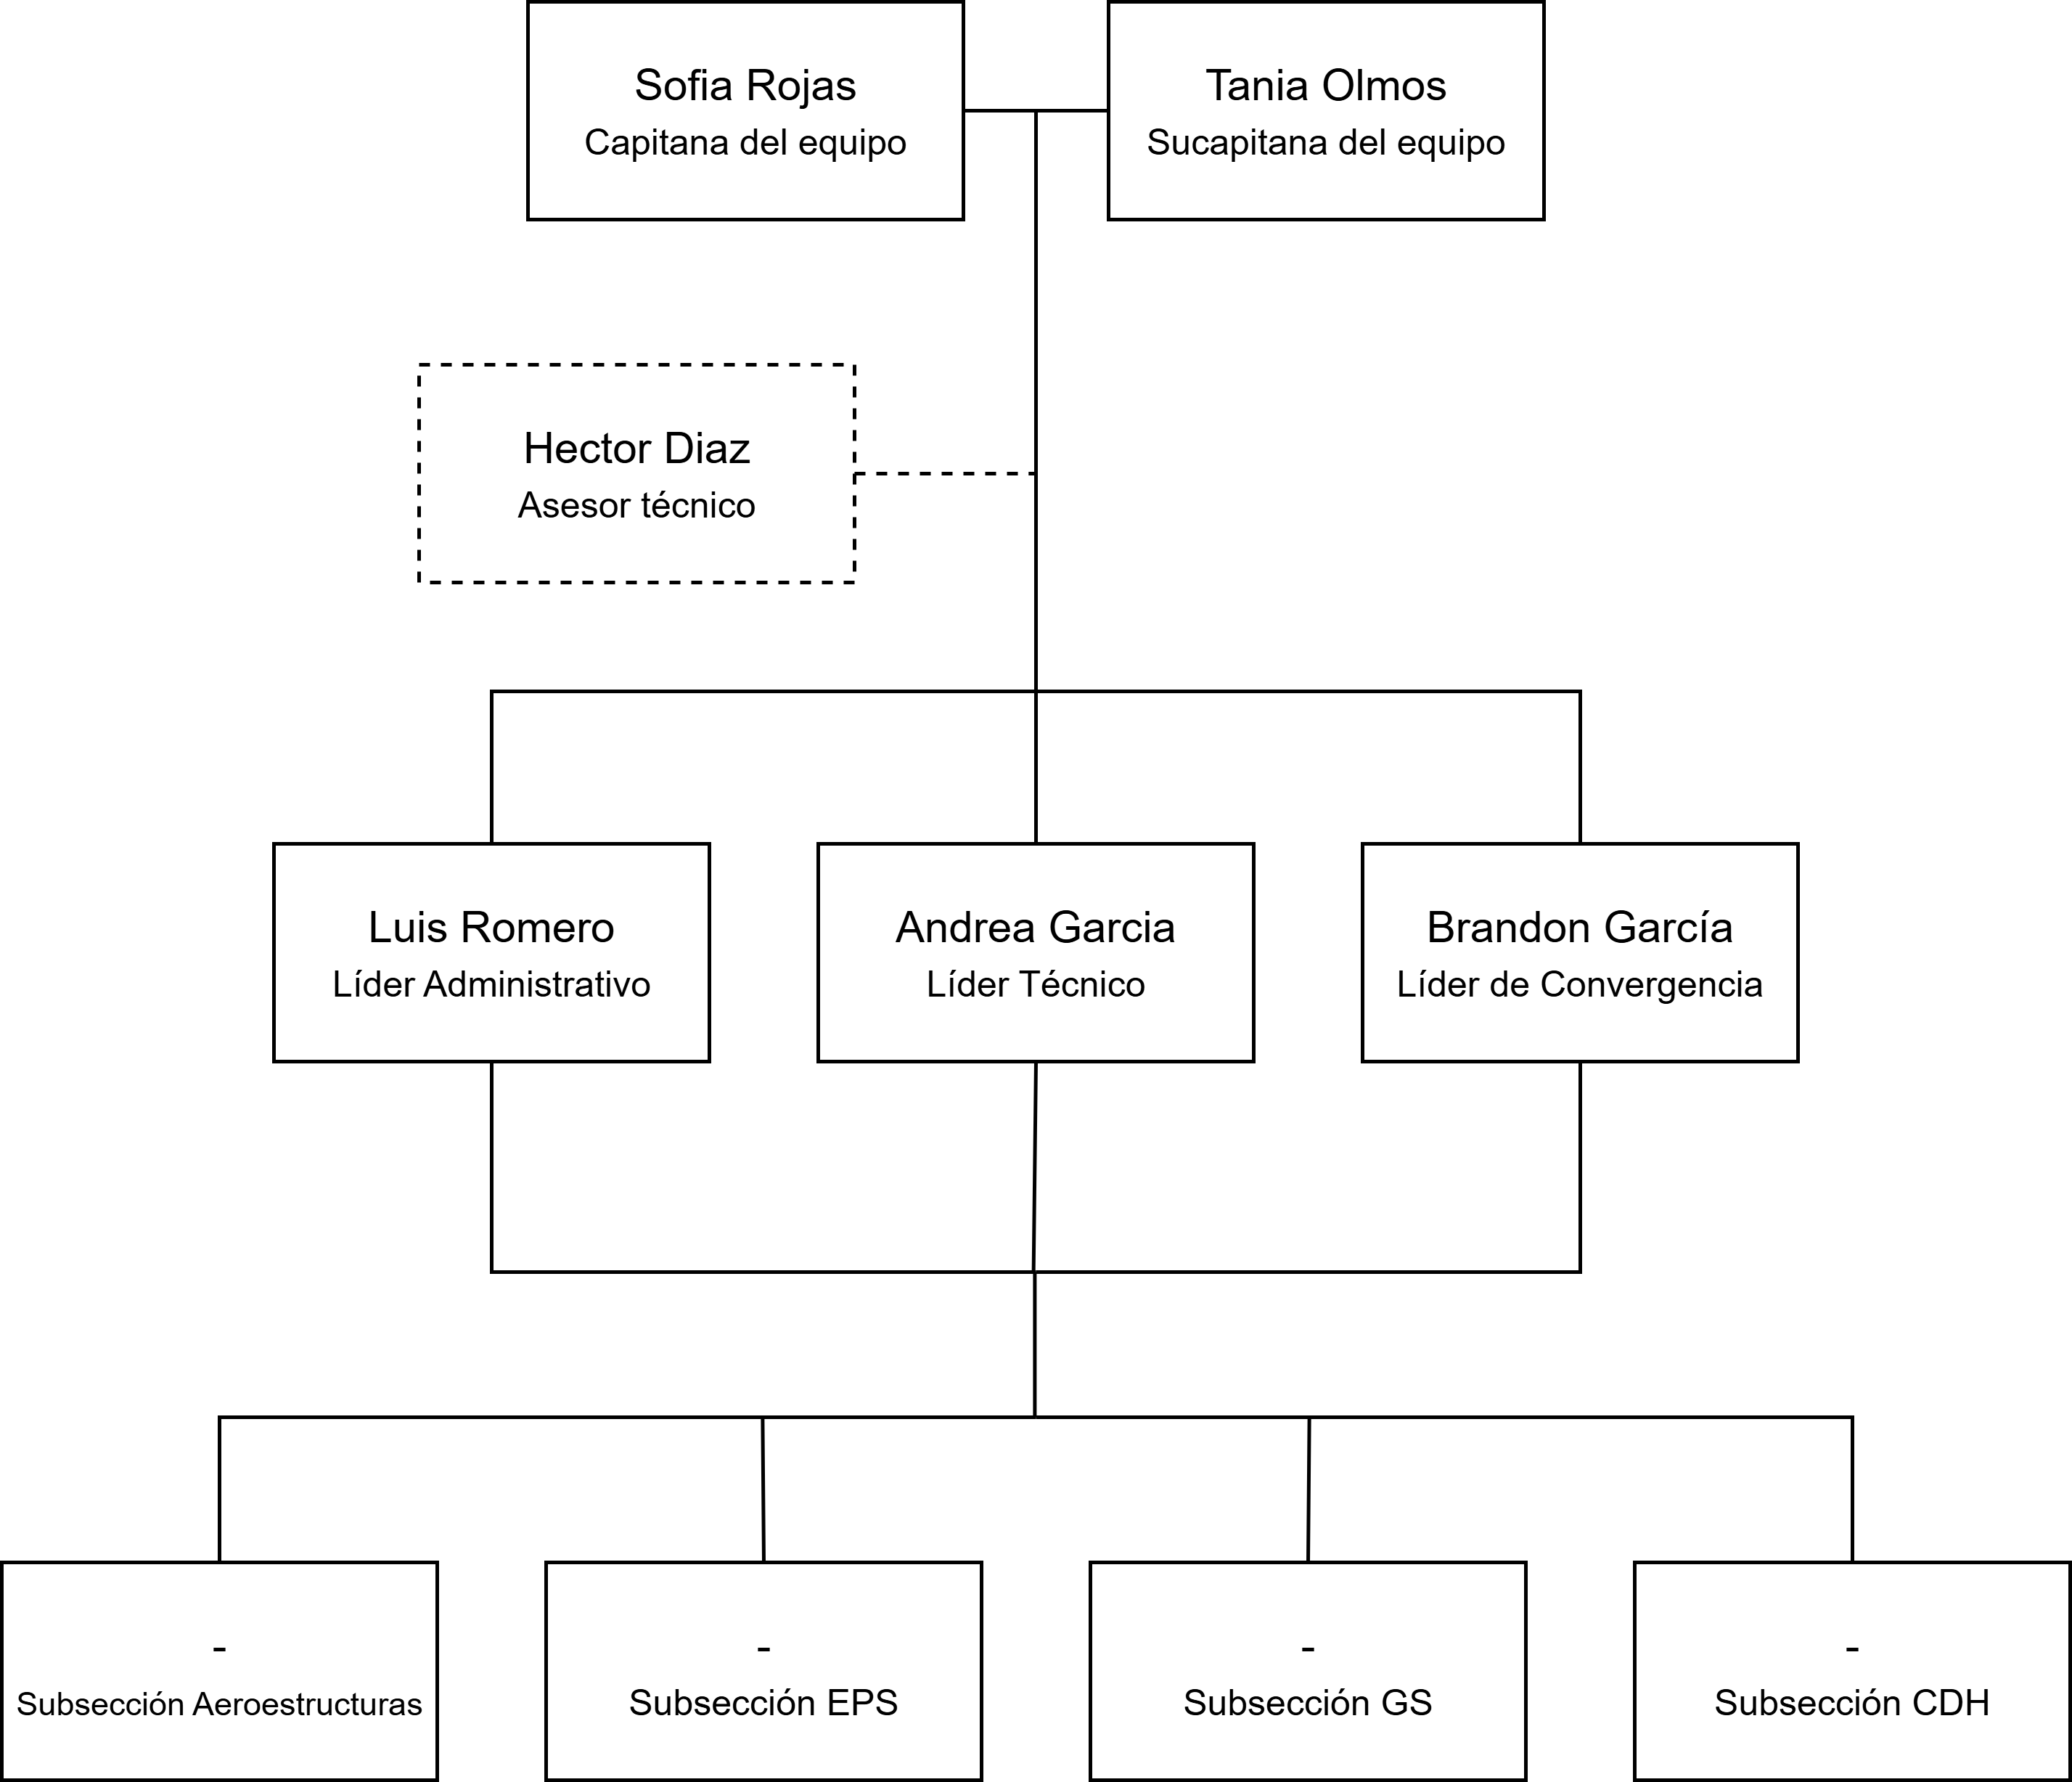
\includegraphics[width=.5\textwidth]{ORG-AYA1-GM-V3.png}}
      \caption{Organigrama Ayahuik 1}
      \label{1}
    \end{figure}
    
    Para la misión Ayahuik 1, el equipo Cuauhtémoc IPN contara con las 2 capitanas del equipo, 
    las cuales se encargaran de coordinar las actividades generales del equipo asi como sus misiones activas, 
    estas son:

    \begin{itemize}
        \item \textbf{Capitana:} Sofia Rojas
        \item \textbf{Subcapitana:} Tania Olmos
    
    \end{itemize}

    De esto se derivara el asesor técnico el cual se encargara de todo el asesoramiento tanto para el funcionamiento del equipo
    como para la correcta realización de la misión sin que este tenga intervención directa, el cual es:

    \begin{itemize}
        \item \textbf{Asesor técnico:} Hector Diaz

    \end{itemize}

    El liderato de la misión AYAHUIK 1 estará a cargo de 3 co-líderes,
    los cuales se encargaran de coordinar el correcto funcionamiento de Cada
    una de las subsecciones del equipo, estos son:

    \begin{itemize}
        \item \textbf{Líder administrativo:} Luis Romero
        \item \textbf{Líder técnico:} Andrea Garcia
        \item \textbf{Líder de convergencia:} Brandon Garcia
    
    \end{itemize}

    De los cuales se derivaran las subsecciones del equipo, las cuales son aeroestructuras, EPS (Electrical Power System), GS (Ground Station) y CDH (Communication and Data Handling).

    \newpage
    \section{Patrocinadores}
    \captionsetup[subfigure]{labelformat=empty}

    \begin{figure}[h!]
    \centering
    \begin{subfigure}[b]{0.3\textwidth}
        \centering
        
\includegraphics[height=3cm]{IPN.png}
        \caption{IPN}
        \label{fig:IPN}
    \end{subfigure}
    \hfill
    \begin{subfigure}[b]{0.3\textwidth}
        \centering
        
\includegraphics[height=3cm]{ESIME.png}
        \caption{ESIME Ticoman}
        \label{fig:ESIME}
    \end{subfigure}
    \hfill
    \begin{subfigure}[b]{0.3\textwidth}
        \centering
        
\includegraphics[height=1.8cm]{FUNDPOL.png}
        \vspace{0.5cm}
        \caption{Fundación Politécnico}
        \label{fig:FUNDPOL}
    \end{subfigure}
    \end{figure}


    \begin{figure}[h!]
    \centering
    \begin{subfigure}[b]{0.3\textwidth}
        \centering
        
\includegraphics[height=2cm]{ALTIUM.png}
        \caption{ALTIUM}
        \label{fig:ALTIUM}
    \end{subfigure}
    \hfill
    \begin{subfigure}[b]{0.3\textwidth}
        \centering
        
\includegraphics[height=1cm]{ALTAIR.png}
        \vspace{0.1cm}
        \caption{ALTAIR}
        \label{fig:ALTAIR}
    \end{subfigure}
    \hfill
    \begin{subfigure}[b]{0.3\textwidth}
        \centering
        
\includegraphics[height=1.2cm]{PCBMEX.png}
        \vspace{0.5cm}
        \caption{PCB México}
        \label{fig:PCBMEX}
    \end{subfigure}
    \end{figure}

    \hspace{0.3cm}
    \begin{figure}[h!]
    \centering
    \begin{subfigure}[b]{0.3\textwidth}
        \centering
        
\includegraphics[height=1.1cm]{SSC.png}
        \vspace{0.2cm}
        \caption{GRUPO SSC}
        \label{fig:SSC}
    \end{subfigure}
    \hfill
    \begin{subfigure}[b]{0.3\textwidth}
        \centering
        
\includegraphics[height=1.5cm]{ANSYS.png}
        \caption{ANSYS}
        \label{fig:ANSYS}
    \end{subfigure}
    \hfill
    \begin{subfigure}[b]{0.3\textwidth}
        \centering
        
\includegraphics[height=1.2cm]{DASSAULT.png}
        \vspace{0.2cm}
        \caption{DASSAULT SYSTEMES}
        \label{fig:DASSAULT}
    \end{subfigure}
    \end{figure}
    
    \hfill


    Gracias por su apoyo, sin ustedes nada de esto sería posible.

    Atte. Cuauhtémoc IPN

    \end{document}
